\section{Brainstorm}

\begin{figure}[H]
\center
 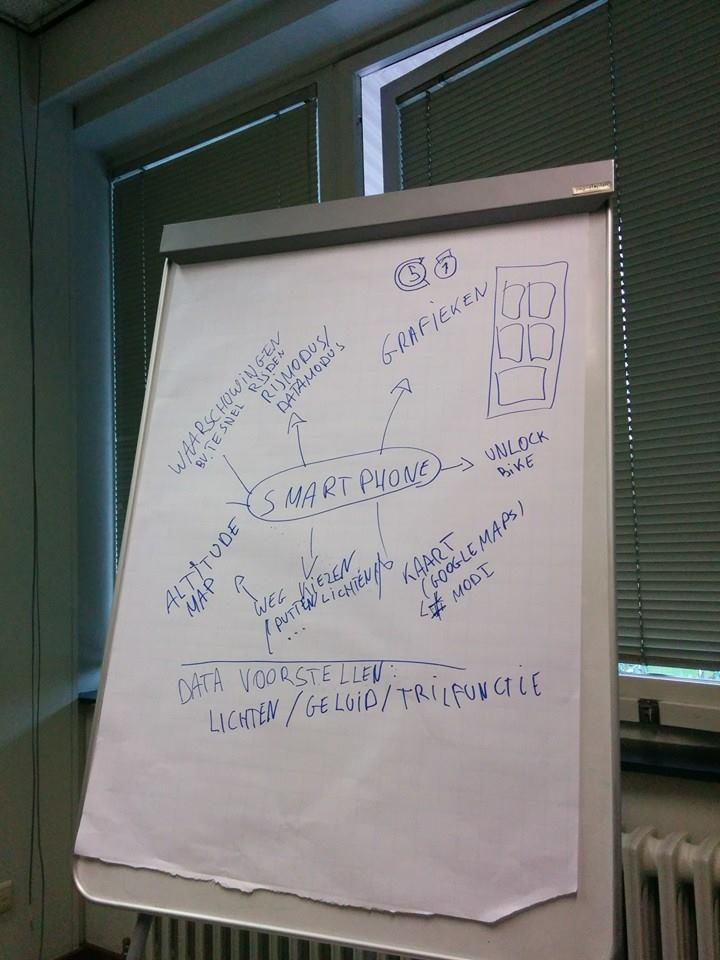
\includegraphics[width=\linewidth]{brainstorm/brainstorm1.jpg}
 \caption{First brainstorm}
 \label{image:ganttchart}
\end{figure}
\begin{figure}[H]
\center
 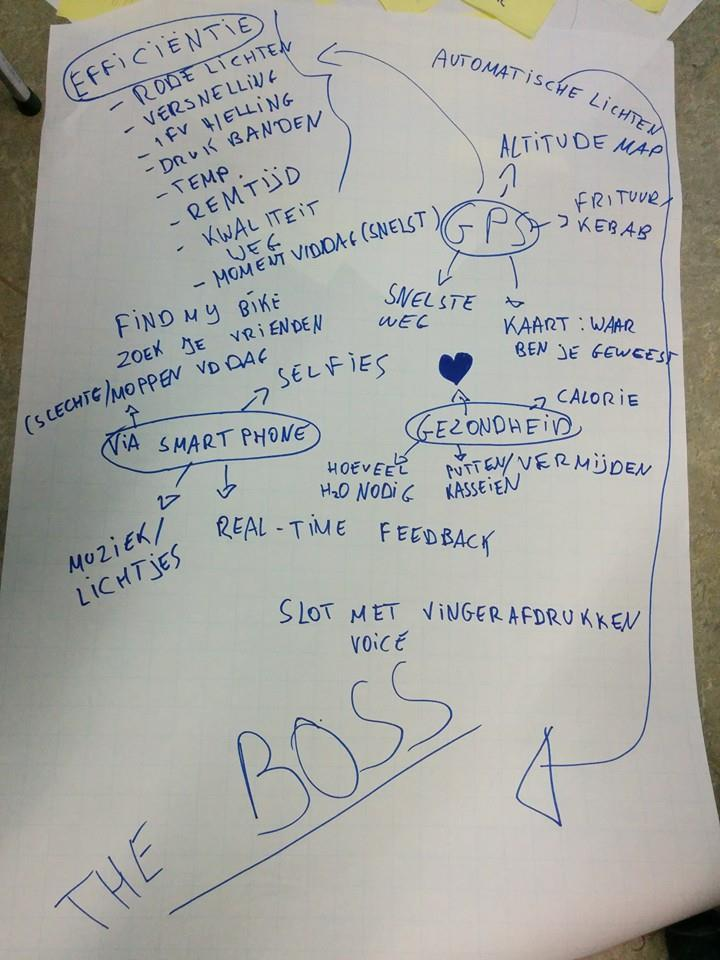
\includegraphics[width=\linewidth]{brainstorm/brainstorm2.jpg}
 \caption{Second brainstorm}
 \label{image:ganttchart}
\end{figure}
A list of all the ideas created during the brainstorm.
\begin{enumerate}
 \item Using a smartphone
 \begin{enumerate}
 \item get real-time feedback
 \item play music/ put on a light
 \item take pictures of yourself/ your surroundings 
 \item easily find where your bike is parked
 \item view in an instance where your friends are
 \end{enumerate}
 \item using a GPS
  \begin{enumerate}
  \item get the fastest way from one point to another
  \item display a card, showing all the places you have been to with your bike. 
  \item Make an altitude map
  \item Easily track the distances you've covered.
  \item display some points of interest ( ex. All the pizza restaurants nearby)
  \end{enumerate}
  \item try to make your trip as efficient as possible
  \begin{enumerate}
  \item avoid red lights, based on your previous bike trips
  \item get a map, displaying the quality of the roads 
  \item find out during which moment of the day you cover a certain way the fastest
  \item get the average time needed to brake
  \item view your speed, based on the altitude difference, the temperature, the hour,...
  \item avoid bad ways 
  \end{enumerate}
  \item monitor your health
  \begin{enumerate}
   \item how many calories have you lost
    \item how much water do you need 
  \end{enumerate}
\end{enumerate}


The initial idea was to use a smartphone, since these devices contain almost all the sensors needed for the project. 
This way, creating an app for Android and iPhone devices would be enough for the concept to be functional. 
The assignment, however, was to incorporate an Arduino Nano and a Raspberry Pi. 
Since using a smartphone, an Arduino and a Raspberry Pi would get a bit too complicated, our team decided against using a smartphone. 
This meant that there would not be any screen attached to the Boss device anymore. 
Real-time communication with the user was therefore no longer possible and functions such as find-your-friends and find-your-bike not doable anymore. 

A lot of the ideas created during the brainstorm, focused on getting an augmented bike. 
This is not what the Boss device was aiming for: the purpose of this project was to create an quantified bike device, without looking at the augmented side of a bike trip. 
Once this goal had been set, a lot of the brainstorm ideas could be thrown overboard: get the fastest way, view your calorie deficit, see how much water you need, locate your friends, get points of interest,...

The idea of trying to avoid red lights seemed very appealing at first, but turned out to be too difficult to implement. It would require an accurate route planner that constantly refreshed, while taking all the red lights in the area into account. A second reason against this idea was the fact that, as a lot of other ideas, it is much more on the augmented than on the quantified side of a bike trip. 